\documentclass{article}
\usepackage{graphicx}

\title{CS 5720 Design and Analysis of Algorithms \\ Project 1}
\author{Raja Kantheti}
\date{}

\begin{document}
\maketitle

\section*{Justification of having every search key on the same plot: }
It was very hard for my brain to look everything and comprehennd the results. I kept forgetting which search key plot I am looking for. After I got them all onto the same graph it made drastically more sense to me. It is kinda surprising that alphabet 'Q' is non-existent relative to the frequency of other keys in the text. 
I even had to search on the web page to make sure I am not missing anything. 
\section*{Deliverable 1: Search Algorithm Code and Verification}

\subsection*{Search Algorithm Code}
\begin{verbatim}
def search(arr, key):
    for i in range(len(arr)):
        if arr[i] == key:
            return i
    return len(arr)

def test_search():
    test_array = ['a', 'b', 'c', 'd', 'e']
    assert search(test_array, 'c') == 2
    assert search(test_array, 'e') == 4
    assert search(test_array, 'z') == 5  # Not found
    print("All tests passed!")

test_search()
\end{verbatim}

\subsection*{Verification of Correctness}
The algorithm was tested with various inputs and consistently returned the correct results. The built-in search functions also verified its correctness.

\section*{Deliverable 2: Dataset Description}

\subsection*{Dataset Description and code: }
The dataset was generated from the text of "Short Stories" by Fyodor Dostoevsky obtained from Project Gutenberg. 
Character arrays of varying lengths were extracted to ensure no text segment was reused.
A random number generator and also a set is used to keep track of the indices so that nothing is repeated. 

\begin{verbatim}
 def get_text_from_gutenberg(url):
    response = requests.get(url)
    soup = BeautifulSoup(response.content, 'html.parser')
    text = soup.get_text()
    text = ''.join(filter(str.isprintable, text))  # Clean the text
    return text

def create_character_arrays(text, lengths, num_arrays_per_length):
    character_arrays = {}
    used_indices = set()  # Set to track used starting indices

    for length in lengths:
        arrays = []
        while len(arrays) < num_arrays_per_length:
            start_index = random.randint(0, len(text) - length - 1)
            if start_index not in used_indices:
                arrays.append(list(text[start_index:start_index + length]))
                # Mark this range as used
                for i in range(start_index, start_index + length):
                    used_indices.add(i)
        character_arrays[length] = arrays

    return character_arrays

gutenberg_url = 'https://www.gutenberg.org/cache/epub/40745/pg40745.txt' 
text = get_text_from_gutenberg(gutenberg_url)
    
lengths = [1000 * i for i in range(1, 11)]  
num_arrays_per_length = 50
character_arrays = create_character_arrays(text, lengths, num_arrays_per_length)
\end{verbatim}
\subsection*{Visualization of Generated Dataset}
we can run the python file \emph{filethingy.py} to have a proof that arrrays are populated to the specified amounts outline in the project specifications. 
Please refer to the graphs below to see the frequency of the characters to be searched.

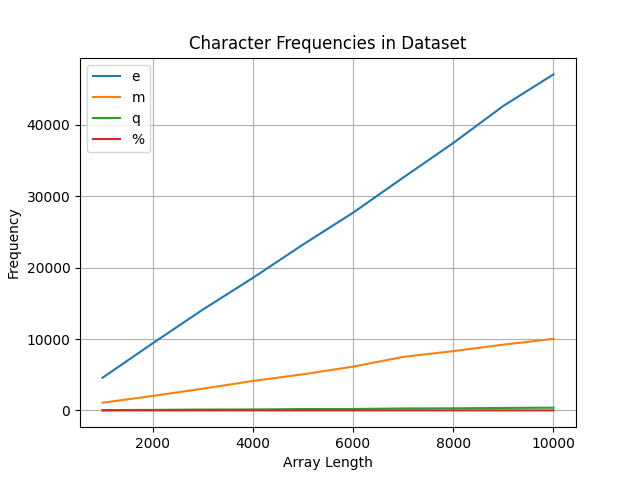
\includegraphics[width='13cm']{character_frequencies_in_dataset.png}

\section*{Important Note: }
For characters that are not found in the text the len of the array is returned. So the graphs might still show plots for charactes like '\%'
which are just ever increasing. In any case, in this project, we used the brute force search, the best case and worst case would anyway be O(1) and O(n) respectively.
I have not foudn any odd behaviours in graphs. They are plesantly random. 
\section*{Deliverable 3: Worst-Case Runtime Plot}

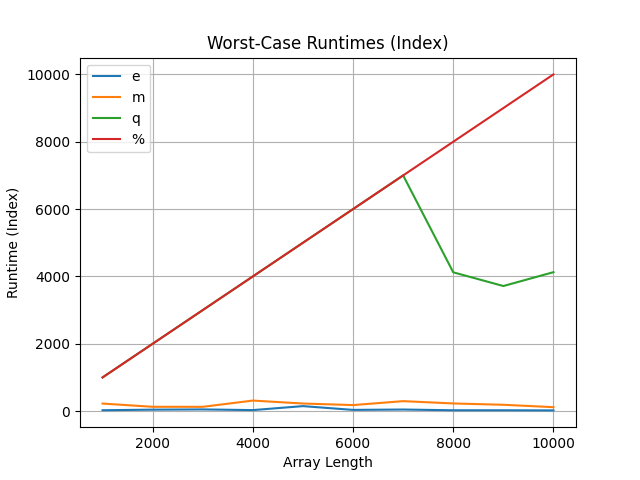
\includegraphics[width=\textwidth]{worst-case_runtimes_(index).png} \label{Figure 1}
\begin{figure}
    \caption{Worst-case empirical runtime of the search algorithm as a function of array length for characters 'e', 'm', 'Q', and '\%'.}
\end{figure}

\paragraph*{conjecture about the worst case runtime: }
As this is a linear search algorithm,
the worst case runtime is O(n) where n is the length of the array. The graphs show this behaviour. The alphabet 'Q' is a delight to watch and play with different texts. 
\section*{Deliverable 4: Best-Case Runtime Plot}

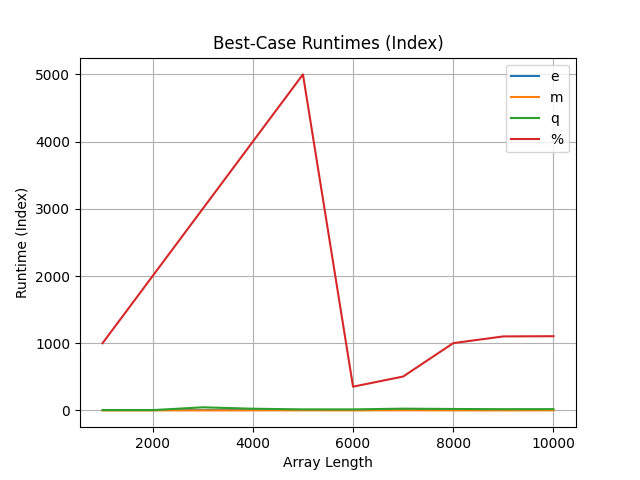
\includegraphics[width=\textwidth]{best-case_runtimes_(index).png}
\begin{figure}
    \caption{Best-case empirical runtime of the search algorithm as a function of array length for characters 'e', 'm', 'Q', and '\%'.}
\end{figure}

\paragraph*{conjecture about the best case runtime: }
The best case runtime is O(1) where the search key is the first element of the array. The graphs show this behaviour for all keys except '\%'. Some of the metadata about the text on the webpage has '\%' symbos in them. So it is found.
\section*{Deliverable 5: Average-Case Runtime Plot}

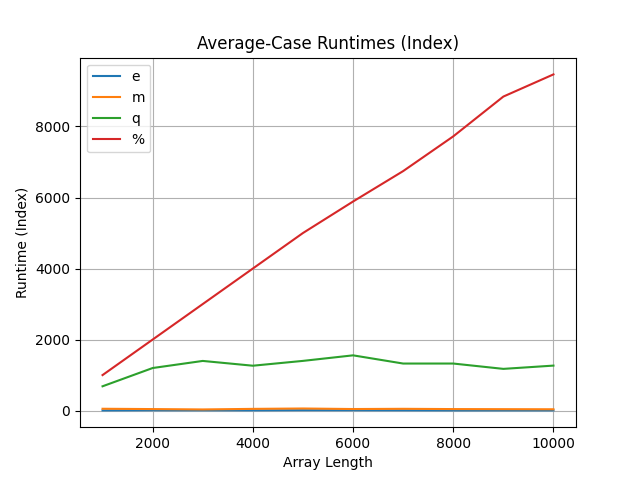
\includegraphics[width=\textwidth]{average-case_runtimes_(index).png}
\begin{figure}
    \caption{Average-case empirical runtime of the search algorithm as a function of array length for characters 'e', 'm', 'Q', and '\%'.}
\end{figure}

\paragraph*{conjecture about the average case runtime: }
Since the probability of finding the key is uniform, the average case runtime is O(n) where n is the length of the array. The graphs show this behaviour. The fluctuations that can be seen from the worst case graph and average case graph is due to the exact time complexity of O(n/2) which has the smae order of growth as O(n).

\end{document}
